\documentclass{report}
\usepackage[margin=1in, paperwidth=8.5in, paperheight=11in]{geometry}
%Math packages%
\usepackage{amsmath}
\usepackage{amsthm}
%Spacing%
\usepackage{setspace}
\onehalfspacing
%Lecture number%
\newcommand{\lectureNum}{8}
%Variables - Date and Course%
\newcommand{\curDate}{January 26, 2017}
\newcommand{\course}{CS 251}
\newcommand{\instructor}{Stephen Mann}
%Defining the example tag%
%\theoremstyle{definition}%
\newtheorem{ex}{Example}[section]
%Setting counter given the lecture number%
\setcounter{chapter}{\lectureNum{}}
%Package to insert code%
\usepackage{listings}
\usepackage{courier}
\usepackage{xcolor}
\lstset { %
    tabsize=2,
    breaklines=true,
    language=C++,
    backgroundcolor=\color{blue!8}, % set backgroundcolor
    basicstyle=\footnotesize\ttfamily,% basic font setting
}
%Package used to draw circuits%
\usepackage{circuitikz}
\begin{document}
%Note title%
\begin{center}
\begin{Large}
\textsc{\course{} | Lecture \lectureNum{}}
\end{Large}
\end{center} 
\noindent \textit{Bartosz Antczak} \hfill
\textit{Instructor: \instructor{}} \hfill
\textit{\curDate{}}
\rule{\textwidth}{0.4pt}
% Actual Notes%
\subsubsection{Shift Left and Right Operations}
The \textbf{shift left} operation multiplies a number by 2
\begin{align*}
0010 &= 2 \\
0100 &= 4 && \text{Shifted to the left; multiplied by 2} \\
1000 &= 8 && \text{Shifted to the left again; multiplied by 2}
\end{align*}
This is very useful because it's a much faster process than simple multiplying.
And intuitively, the \textbf{shift right} operation divides a number by 2 (for this operation, we must also duplicate the top bit when shifting)
\begin{align*}
0110 &= 6 \\
0011 &= 3 && \text{Shift to the right and duplicated top bit; divided by 2} \\
\end{align*}
This division approach drops any remainders and returns only the value (e.g., dividing 0011 = 3 by two will yield 0001 = 1.  Dividing 0101 = 5 by two will yield 0010 = 2).
\subsubsection{Multiplication on Binary Numbers}
When we multiply binary numbers, we use the same approach we use to multiply base-10 numbers. Working with our ALU, we'll follow an algorithm to easily multiply numbers (an example is shown):
\begin{figure}[ht]
\begin{center}
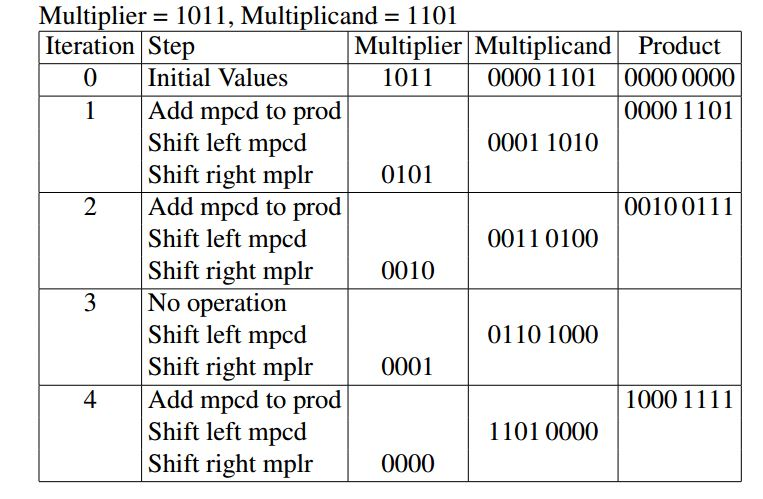
\includegraphics[scale=0.45]{multiplication_example.jpg}
\end{center}
\caption{Source: Multiplying $1011 \times 1101$. Courtesy of Prof. Mann's slides.}
\end{figure}\newpage
\noindent The algorithm works using these following steps:
\begin{enumerate}
\item Consider three initial values: your multiplier, multiplicand, and final product (which is initially 0000 0000)
\item Add the multiplicand to the product, then shift the multiplicand to the left and the multiplier to the right
\item Repeat this process until the multiplier is zero
\end{enumerate}
\subsubsection{Representing Numbers that aren't Integers}
We'll represent these kinds of numbers using a pseudo scientific notation. Our scientific notation will be in base 2. We'll store this in our binary string using the IEEE 754 standard:
\begin{figure}[ht]
\begin{center}
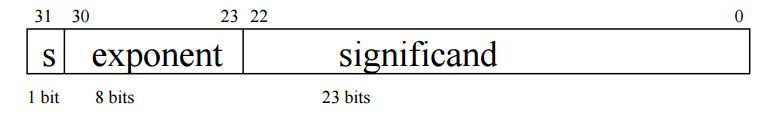
\includegraphics[scale=0.65]{scientific_notation.jpg}
\end{center}
\caption{Source: The template for representing a number in scientific notation using the IEEE 754 standard for a 32-bit string. Courtesy of Prof. Mann's slides.}
\end{figure}\\
The above value is represented as $(-1)^\mathrm{S} \times (1.\mathrm{significand}) \times 2^{\mathrm{(Exponent}\,-\,\mathrm{Bias})}$
%END%
\end{document}